%\usepackage{amsmath}
%\usepackage{hyperref}
%\usepackage{amsthm}
%\usepackage{graphicx}
\documentclass[journal, a4paper]{IEEEtran}
\usepackage[italian]{babel}
\usepackage{booktabs}
\usepackage{siunitx}%Questo serve a caricare il pacchetto delle unità di misura del sistema internazionale%
\usepackage[utf8]{inputenc}
\usepackage{graphicx} 
\usepackage{url}
\usepackage{amsmath}
\usepackage{amssymb}


\usepackage{keyval}
\usepackage{xcolor}
\usepackage{caption}
\usepackage{tikz}
\usepackage{circuitikz}
\usepackage{authblk}
%\usepackage{hyperref}

\begin{document}


% Define document title and author
	\title{Tecnologie Digitali - Logbook Week 6}
	\author[1]{Salvatore Bottaro}
		\author[2]{Lorenzo M. Perrone}
		\affil[1]{\texttt{salvo.bottaro@hotmail.it}}
		\affil[2]{\texttt{lorenzo.perrone.lmp@gmail.com}}
	\markboth{Tecnologie Digitali - Di Lieto}{}
	\maketitle
	
\begin{abstract}
	Logbook di laboratorio di Tecnologie Digitali, a.a. 2015/2016. Week 6.
\end{abstract}

\section{Grandezze fotometriche}

In tabella \ref{tab:foto} sono mostrate le grandezze fotometriche impiegate con relativa unità di misura.

\begin{table}[htp]
\centering
\caption{Grandezze fotometriche.}
\label{tab:foto}
\begin{tabular}{|c|c|c|}
\hline 
Grandezza & Unità SI & Unità fotometrica \\ 
\hline 
Flusso luminoso & W & lumen (lm) \\ 
\hline 
Intensità luminosa & W/sr & candela (cd) \\ 
\hline 
Luminanza & W/(sr m$^2$) & nit = cd/m$^2$ \\ 
\hline 
Illuminamento & W/m$^2$ & lux \\ 
\hline 
\end{tabular} 
\end{table}

Un'unità alternativa per l'illuminamento è il foot-candle (fc) di origine anglosassone, con 1 fc = 10.764 lux.

\section{Fotodiodo e sue specifiche}

\subsection{Hm. 1}

Nel documento \textit{Photodiode Technical Information} della \textit{Hamamatsu} è possibile leggere alcune definizioni tecniche di parametri presenti nei datasheet. 

\begin{itemize}
\item Risposta spettrale: la relazione fra le sensitività fotoelettrica e la lunghezza d'onda espressa in termini di efficienza quantica, fotosensività $\dots$ ;
\item Fotosensitività (S): rapporto fra la potenza incidente sul dispositivo (W) e la fotocorrente generata (A);
\item Efficienza quantica (QE): il rapporto fra il numero di elettroni o buche rilevabili come fotocorrente e il numero di fotoni incidenti. Il QE è espresso in percentuale ed è legato alla fotosensitività dalla relazione:
\begin{equation}
QE = \frac{S \cdot 1240}{\lambda} \cdot 100 [\%]
\end{equation}
con $\lambda$ in nm;
\item Corrente di corto circuito (Isc), tensione a circuito aperto (Voc): la Isc è la fotocorrente che scorre nel dispositivo in modalità fotoconduttiva, ovvero quando il dispositivo è corto circuitato. La Voc è la tensione generata dal fotodiodo a circuito aperto;
\item Dark current ($I_D$), resistenza di shunt (Rsh): la $I_D$ è la corrente che scorre nel fotodiodo quando non è esposto alla luce e vi è applicata una tensione negativa ed è un'importante fonte di rumore quando al fotodiodo è applicata una tensione inversa. Negli altri casi si deve tenere della Rsh, ovvero il rapporto $\frac{V}{I}$ in prossimità di 0 V definita da:
\begin{equation}
Rsh = \frac{10[mV]}{I_D} [\Omega]
\end{equation}
dove $I_D$ è la dark current a 10 mV;
\item Terminal Capacitance ($C_t$): la giunzione PN del fotodiodo ha una capacità effettiva che costituisce il fattore principale nel determinare il tempo di risposta del fotodiodo;
\item Tempo di salita (tr): tempo di risposta del diodo ad un segnale a scalino ed è definito come il tempo necessario per passare dal 10 $\%$ al 90 $\%$ del valore costante di output;
\item Cut-off frequency (fc): misura del tempo di risposta del fotodiodo ad un segnale luminoso sinusoidale. Si definisce come la frequenza a cui l'output diminuisce di 3 dB rispetto a 100 kHz (con resistenza di carico di 50 $\Omega$ e diodo laser di 830 nm). Fra tempo di salita e cut-off frequency vale la relazione:
\begin{equation}
tr = \frac{0.35}{fc};
\end{equation}
\item Noise Equivalent Power (NEP): il NEP è definito come la potenza luminosa incidente necessaria per ottenere un rapporto segnale-rumore pari a 1. Nei datasheet il NEP è riferito alla lunghezza di picco $\lambda _p$. Analiticamente:
\begin{equation}
NEP[W/Hz^{\frac{1}{2}}]=\frac{Noise ~ current \,[A/Hz^{\frac{1}{2}}]}{Fotosensitivit\textit{à} ~ a ~\lambda _p [A/W]};
\end{equation}
\item Massima tensione inversa ($V_R$ MAX);
\item Detectivity (D$^*$): D è il reciproco del NEP e misura la capacità di rilevare un segnale. Poiché il NEP è proporzionale alla radice dell'area sensibile, moltiplicando D per tale radice si ottiene un indicatore della capacità di rilevare i segnali indipendente dalle dimensioni del dispositivo:
\begin{equation}
D^* = \frac{(Area ~ sensibile \,[cm^2])^{\frac{1}{2}}}{NEP}.
\end{equation}
\end{itemize}
In figura \ref{fig:curcar} sono mostrate le curve caratteristiche del fotodiodo al variare della luminosità incidente. Poiché l'elettrone e la buca generate dall'interazione radiazione materia nella regione di svuotamento della giunzione, a causa del campo elettrico presente nella regione stessa diretto dalla regione n alla regione p, sono spinti rispettivamente nella zona n e p, la corrente da essi generata si somma alla reverse current dei portatori minoritari. Questo fa sì che all'aumentare della luminosità la curva caratteristica trasli verso il basso di una quantità data da:
\begin{equation}
I = \eta \, \frac{We}{h\nu}
\end{equation}
dove $\eta$ è l'efficienza quantica, ovvero la probabilità che un fotone incidente generi una coppia elettrone-buca che contribuisca alla fotocorrente.
\begin{figure}[htp]
\centering
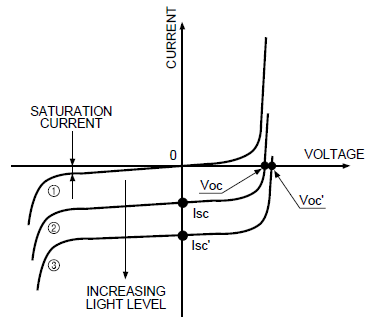
\includegraphics[scale=.6]{curve_car_phdiode}
\caption{Curve caratteristiche del fotodiodo al variare della luminosità incidente.}
\label{fig:curcar}
\end{figure}

\section{Fotodiodo VTB8440BH}

Dal datasheet del fotodiodo si possono leggere le specifiche in tabella \ref{tab:spec}.

\begin{table}[htp]
\centering
\caption{Specifiche del fotodiodo VTB8440BH}
\label{tab:spec}
\begin{tabular}{|c|c|c|}
\hline 
Grandezza & Test conditions & Valore tipico \\ 
\hline 
$I_{SC}$ & H = 100 fc, 2850 K & 5 $\mu$A \\ 
\hline 
$V_{OC}$ & 2850 K & 420 mV \\ 
\hline 
$I_D$ & H = 100 fc, 2850 K & 2 nA (max) \\ 
\hline 
$R_{SH}$ & H = 0, V = 10 mV & 70 M$\Omega$ \\ 
\hline 
$C_J$ & H = 0, V = 0 & 1 nF \\ 
\hline 
$\lambda _p$ &  & 580 nm \\ 
\hline 
NEP &  & 1.1 $\cdot$ $10^{-13}$ W/$\sqrt{Hz}$ \\ 
\hline 
D$^*$ &  & 2.2 $\cdot$ $10^{12}$ cm$\sqrt{Hz}$/W \\ 
\hline 
\end{tabular} 
\end{table}

Le prime prove sono state fatte collegando direttamente il fotodiodo al multimetro. Abbiamo dapprima impiegando il multimetro come voltmetro studiando quindi la risposta del fotodiodo in modalità fotovoltaica. Abbiamo individuato anodo e catodo del fotodiodo semplicemente guardando in che modo bisognava collegarlo per avere tensioni positive, dal momento che in caso di esposizione alla luce in modalità fotovoltaica la d.d.p. fra anodo e catodo deve essere positiva. In particolare abbiamo individuato il catodo (-) in corrispondenza di un forellino presente sul dispositivo. Abbiamo effettuato diverse misure dell'intensità luminosa in varie condizioni, in tabella \ref{tab:ill} abbiamo riportato i risultati con le relative condizioni.

\begin{table}[htp]
\centering
\caption{$V_{oc}$ (mV) in varie condizioni.}
\label{tab:ill}
\begin{tabular}{|c|c|}
\hline 
Condizione & $V_{oc}$ (mV) \\ 
\hline 
Luce lab. & 388 $\pm$ 1 \\ 
\hline 
Flash cellulare & 534 $\pm$ 5 \\ 
\hline 
Lente di ingrandimento & 400 $\pm$ 2 \\ 
\hline
Coperto con foglio di carta & 2 $\pm$ 1 \\ 
\hline  
\end{tabular} 
\end{table}

Per vedere come la risposta fotovoltaica dipenda dall'intensità luminosa abbiamo posizionato il flash della fotocamera del cellulare sul fotodiodo a varie distanze, tenendo conto che l'intensità luminosa è quadratica nella distanza (anche se non è proprio così nel caso del flash del cellulare), coprendo in parte cellulare e fotodiodo con un foglio per schermare la luce del laboratorio (misura effettivamente non essenziale). I dati sono riportati in figura \ref{fig:illum} e mostrano chiaramente come l'andamento sia non lineare. I valori ottenuti sono comunque dello stesso ordine di grandezza della $V_{oc}$ tipica riportata nel datasheet.

\begin{figure}[htp]
\centering
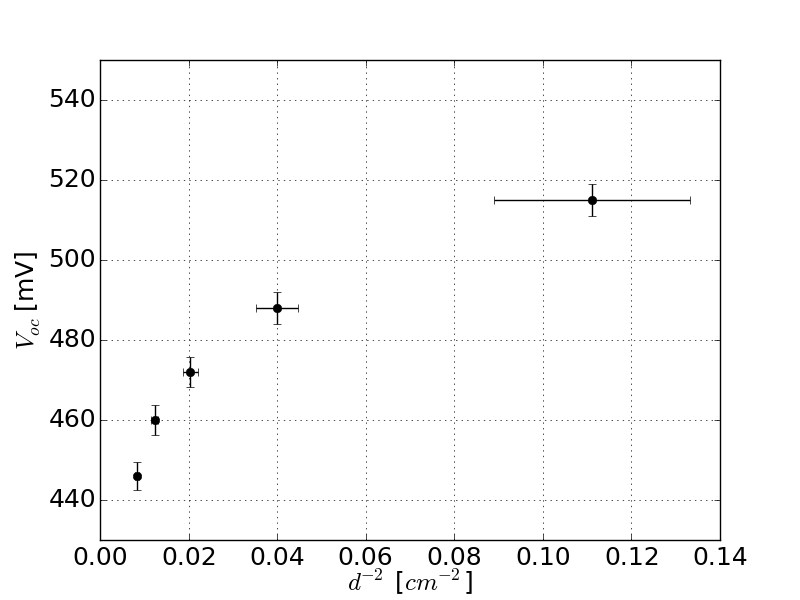
\includegraphics[scale=.4]{illum2}
\caption{Grafico di $V_{oc}$ in funzione dell'inverso della distanza al quadrato del flash.}
\label{fig:illum}
\end{figure}

Impiegando il multimetro come amperometro, in buona approssimazione i capi del fotodiodo sono cortocircuitati per cui si ha che esso lavora in modalità fotoconduttiva. In questa modalità si dovrebbe avere una dipendenza lineare dall'illuminazione, e quindi nelle ipotesi precedenti lineare con il quadrato della distanza del flash del cellulare impiegato. Abbiamo collegato l'anodo del fotodiodo all'ingresso del multimetro, per cui le crrenti osservate dovrebbero essere negative. Di fatti quello che abbiamo osservato sono state proprio correnti negative, per cui nel seguito ci si riferirà ai valori assoluti. Il valore della fotocorrente nel diodo alla luce del laboratorio, nella nostra postazione, vale I = (1.12 $\pm$ 0.01) $\mu$A, mentre il valore tipico riportato ne datasheet è 5 $\mu$A. Con le stesse modalità di prima abbiamo indagato la dipendenza della corrente dalla distanza, ottenendo il grafico in figura \ref{fig:illum_cor} in cui è evidente un andamento decisamente più lineare.

\begin{figure}[htp]
\centering
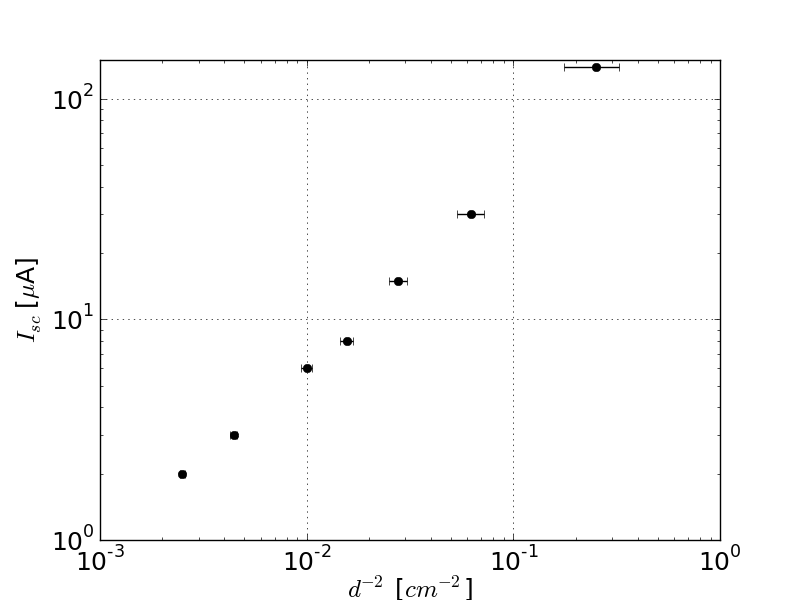
\includegraphics[scale=.4]{illum_cor2}
\caption{Grafico di $I_{sc}$ in funzione dell'inverso del quadrato della distanza.}
\label{fig:illum_cor}
\end{figure}

Dopo queste prove preliminari, abbiamo realizzato sulla breadboard il circuito in figura \ref{fig:es4}. In queste condizioni, per le regole d'oro dell'opamp il fotodiodo è in modalità fotoconduttiva poiché i suoi terminali sono alla stessa differenza di potenziale, per cui la resistenza di carico elevata consente di tradurre in tensioni che si possono agevolmente misurare delle correnti piccole come le fotocorrenti.

\begin{figure}[htp]
\centering
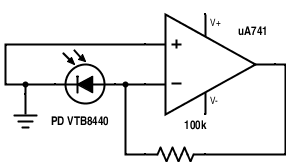
\includegraphics[scale=.6]{ES4}
\caption{Circuito realizzato per la misura delle fotocorrenti.}
\label{fig:es4}
\end{figure}

Utilizzando il VI \texttt{ACQUIS$\_$BASE$\_$2015} abbiamo misurato l'illuminazione del laboratorio. I dati sperimentali sono in figura \ref{fig:illnoncop}.

\begin{figure}[htp]
\centering
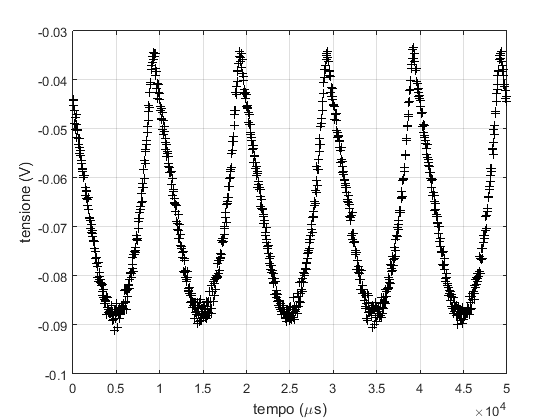
\includegraphics[scale=.5]{es4_noncoperto}
\caption{Illuminazione del laboratorio rilevata dal fotodiodo in funzione del tempo.}
\label{fig:illnoncop}
\end{figure}

Come si vede le tensioni sono negative, questo perché la fotocorrente scorre verso l'uscita dell'opamp. Il segnale osservato è periodico ad una frequenza di 100 Hz, questo perché le lampade fluorescenti del laboratorio sono alimentate da corrente alternata a 50 Hz e dal momento che l'intensità è quadratica nei campi si ottiene una frequenza principale doppia (più armoniche superiori). Il fatto che il segnale non vada a zero quando è dovuto al fatto che i tempi di reazione del gas nelle lampade sono maggiori del periodo della corrente di alimentazione, per cui non tutte le molecole del gas sono diseccitate quando la corrente è nulla. Non può essere infatti un problema di offset del fotodiodo poiché il segnale che si ottiene coprendo con dei fogli il fotodiodo varia in un intervallo compreso fra -2 mV e 6 mV, come si vede in figura \ref{fig:illumfogli}. Calcolando il valore medio e lo scarto quadratico medio si ottiene una misura dell'offset di (2217 $\pm$ 2) $\mu$V.

\begin{figure}[htp]
\centering
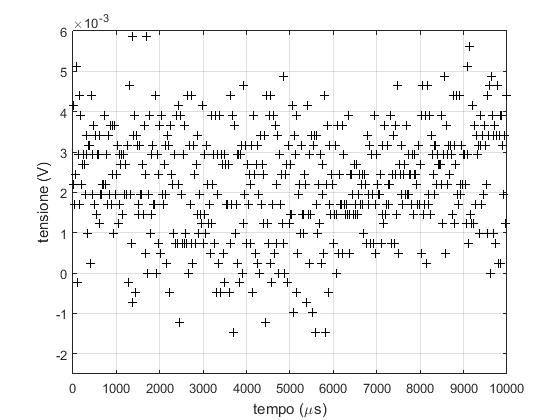
\includegraphics[scale=.5]{es4_copertofoglio_0-01_50k}
\caption{Segnale rilevato coprendo il fotodiodo con dei fogli.}
\label{fig:illumfogli}
\end{figure} 

Abbiamo infine ripetuto la misura dell'illuminazione del laboratorio con una lente di ingrandimento, facendo convergere il più possibile la luce della lampada sul fotodiodo. Come si vede in figura \ref{fig:lente}, si ottiene un segnale praticamente identico a quello di figura \ref{fig:illnoncop}, ma traslato verso il basso di circa 30 mV e con un'ampiezza di 20 mV circa maggiore, corrispondente al passaggio di più corrente nel fotodiodo e quindi ad un'illuminazione maggiore.

\begin{figure}[htp]
\centering
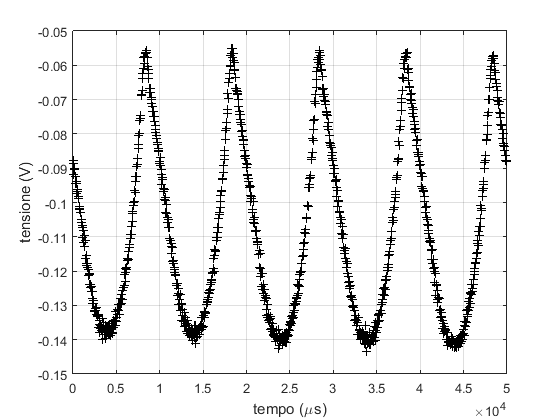
\includegraphics[scale=.5]{es4_noncoperto_lente_0-05_20k}
\caption{Illuminazione del laboratorio con lente di ingrandimento.}
\label{fig:lente}
\end{figure}

\subsection{Hm. 2}
Dal datasheet il grafico che consente la conversione fra corrente e illuminazione è quello riportato in figura \ref{fig:relcur}. Sull'asse delle coordinate viene riportata la corrente relativa, ovvero 100 volte il rapporto fra la fotocorrente misurata e il valore tipico di 5 $\mu$A riportato sul datasheet. A I$_{rel}$ = 5 $\mu$A corrisponde un'illuminazione di 100 fc.

\begin{figure}[htp]
\centering
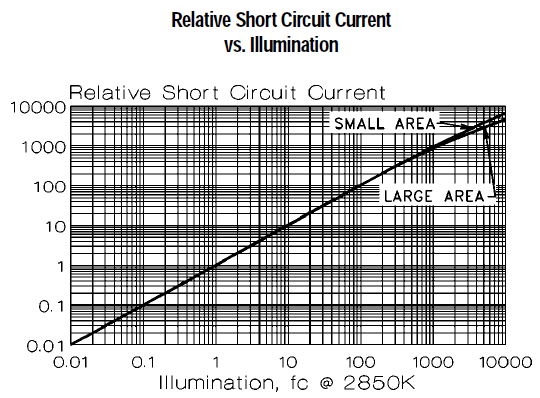
\includegraphics[scale=.5]{current}
\caption{Illuminazione vs corrente relativa.}
\label{fig:relcur}
\end{figure}

Il valor medio della corrente nel fotodiodo vale (0.674 $\pm$ 0.002) $\mu$A che dal grafico \ref{fig:relcur} corrisponde un'illuinazione di circa 13-14 fc.

\section{Fotodiodo e LED}

Poiché dal datasheet emerge che il fotodiodo ha la migliore risposta per $\lambda$ = 580 nm, abbiamo deciso di usare un LED HLPM-C315 che ha lunghezza d'onda di picco a 585 nm. Come si vede dalla figura \ref{fig:hlmp} tratta dal datasheet del LED, la luminosità cresce linearmente con la corrente a partire dai 12-13 mA, per cui nel seguito abbiamo fatto attenzione a mantenerci in questo range.

\begin{figure}[htp]
\centering
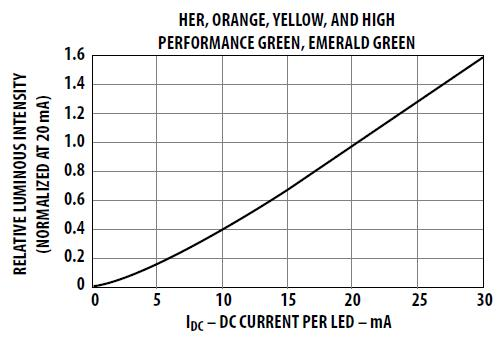
\includegraphics[scale=.6]{hlmpc315}
\caption{Intensità luminosa emessa dal LED in funzione della corrente.}
\label{fig:hlmp}
\end{figure}

Abbiamo montato sulla breadboard il circuito di alimentazione del LED. Abbiamo scelto come resistenza di carico R = 215 $\Omega$ $\pm$ 0.8 $\%$, in modo tale da poter raggiungere le correnti di lavoro. Tramite il VI \texttt{$Vin\_Vout\_2C$} abbiamo individuato il range di tensioni da applicare al LED per ottenere le correnti di interesse. Dai dati in tabella \ref{tab:curLED} si vede che per tensioni comprese fra 5 e 6 V le correnti rientrano nella regione di linearità del LED, inoltre si vede anche come la corrente dipenda linearmente dalla tensione $V_{in}$ di alimentazione.

\begin{table}
\centering
\caption{Correnti nel LED all'aumentare di $V_{in}$.}
\label{tab:curLED}
\begin{tabular}{|c|c|c|}
\hline 
$V_{in}$ (V) & $V_R$ (V)& $I_{LED}$ (mA)\\ 
\hline 
5 & 3(0) & 14 \\ 
\hline 
5.2 & 3.191(0)& 14.8 \\ 
\hline 
5.4 & 3.3812(6) & 15.7 \\ 
\hline 
5.6 & 3.569(0) & 16.6 \\ 
\hline 
5.8 & 3.7596(5) & 17.5 \\ 
\hline 
6 & 3.95(0) & 18.4 \\ 
\hline 
\end{tabular} 
\end{table}

Il LED è stato collegato ad un cavo flessibile in modo tale da poterlo posizionare direttamente sul fotodiodo. Tramite il VI \texttt{$PD\_LED$} abbiamo tracciato la caratteristica $I_{LED}~ vs~I_{PD}$, impiegando un range di tensioni da 0 V a 6 V. In figura \ref{fig:es8} sono mostrati i dati sperimentali in cui è evidente, già per basse correnti, un andamento lineare. Questo è in accordo con la risposta lineare del fotodiodo e con la dipendenza lineare dell'illuminazione emessa dal LED dalla tensione applicata, soprattutto per alte correnti.

\begin{figure}[htp]
\centering
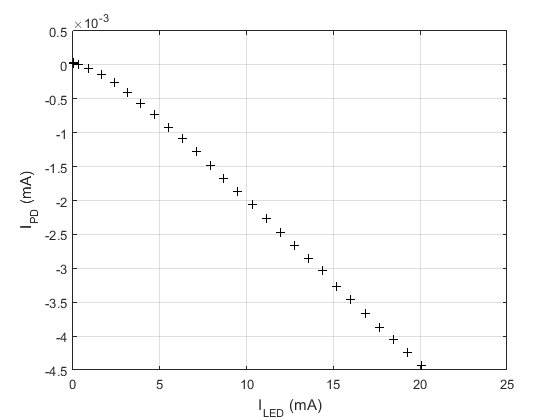
\includegraphics[scale=.5]{es8_0-6_30mis_mejo}
\caption{Caratteristica $I_{LED}~ vs~I_{PD}$ con intervallo di tensioni 0-6 V}
\label{fig:es8}
\end{figure}

\subsection{Hm. 3}
In figura \ref{fig:sens} si vede il grafico della sensitività del fotodiodo in funzione della lunghezza d'onda. Questo consente di tradurre i dati sulla corrente in termini di illuminamento del fotodiodo. Poiché il LED emette ad una lunghezza d'onda di 583 $\pm$ 15 nm, si può stimare dal grafico \ref{fig:sens} una sensitività di 0.23 $\pm$ 0.01 (A/W). 

\begin{figure}[htp]
\centering
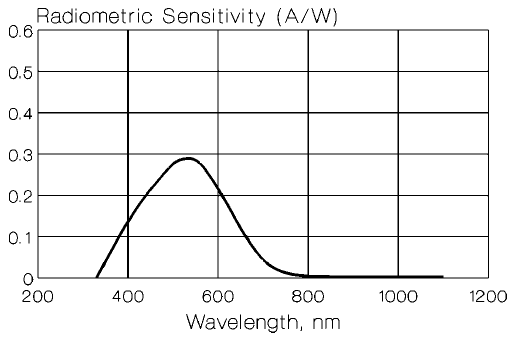
\includegraphics[scale=.5]{sensitivity}
\caption{Sensitività del fotodiodo in funzione della lunghezza d'onda.}
\label{fig:sens}
\end{figure}

Poiché 1 W vale 683 lm a 555 nm di lunghezza d'onda e dal momento che la lunghezza d'onda impiegata è simile, si può assumere valido questo fattore di conversione. Il grafico con l'illuminamento in funzione della corrente nel LED è in figura \ref{fig:illum_cor}.

\begin{figure}[htp]
\centering
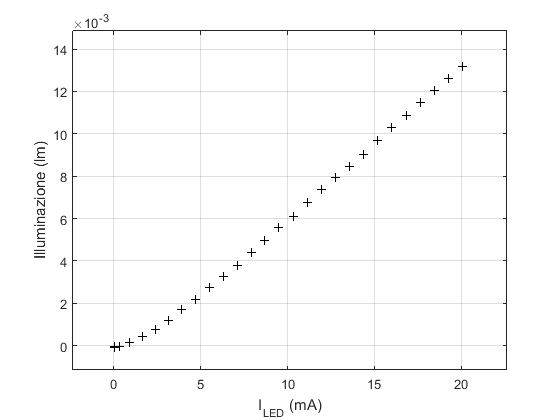
\includegraphics[scale=.5]{illum_cur}
\caption{Illuminazione sul fotodiodo in funzione della corrente nel LED.}
\label{fig:illum_cor}
\end{figure}

Abbiamo studiato la dipendenza dell'intensità luminosa al variare della distanza del LED. Per fare questo abbiamo avvolto un foglio di carta su se stesso e infilato dentro il LED, dopodiché abbiamo poggiato il rotolo sul fotodiodo e avviato il VI \texttt{$PD\_LED$} aumentando progressivamente la distanza del LED. In figura \ref{fig:dist} sono riportate le caratteristiche $I_{LED}~ vs~I_{PD}$ al variare della distanza.

\begin{figure}[htp]
\centering
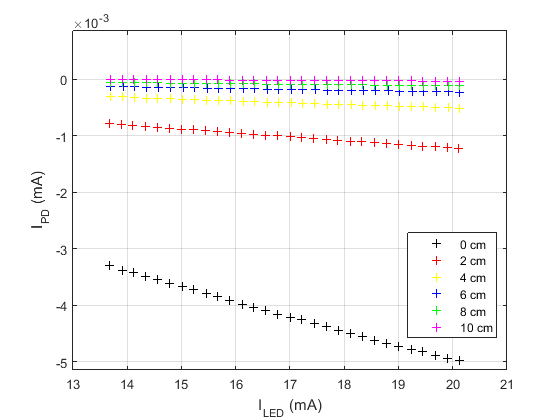
\includegraphics[scale=.6]{distance}
\caption{Caratteristica $I_{LED}~ vs~I_{PD}$ al variare della distanza del LED}
\label{fig:dist}
\end{figure}

L'ipotesi più semplice per quanto riguarda la dipendenza intensità-distanza è una legge del tipo:

\begin{equation}
\label{eqn:fit}
I = a + \frac{b}{(x-c)^2}
\end{equation}

che rende conto del fatto che il fotodiodo potrebbe avere un offset (parametro a) e che per x = 0 I resti finita (idealmente quello che si osserva ponendo il LED a contatto con il fotodiodo). Per verificare questo andamento abbiamo scelto gli ultimi dati di ciascuna curva stimando l'errore sulla corrente tramite:

\begin{equation}
\Delta I = \sqrt{(\frac{\Delta V}{R})^2 + (\frac{I\, \Delta R}{R})^2}
\end{equation}

In figura \ref{fig:discor} è riportato il fit, mentre in tabella \ref{tab:fit} i parametri fittati secondo la legge \ref{eqn:fit}.

\begin{figure}[htp]
\centering
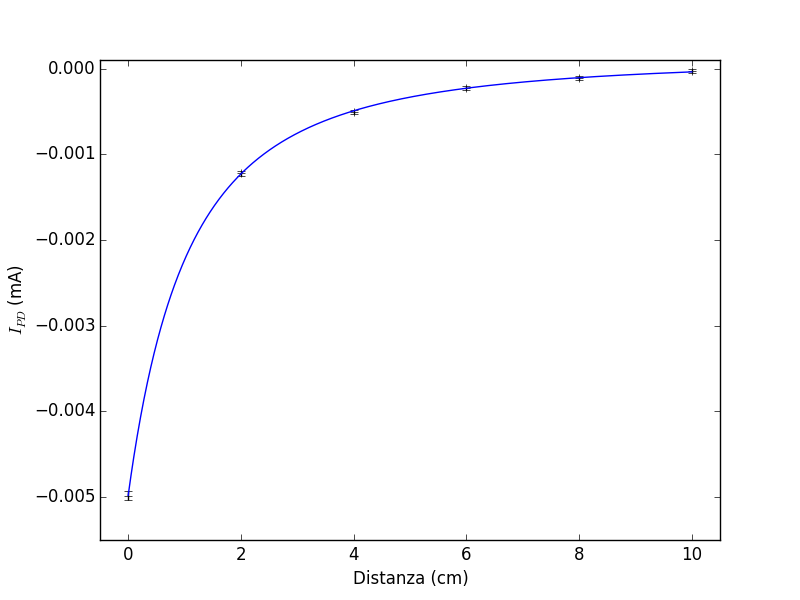
\includegraphics[scale=.4]{distanza_cor}
\caption{Fit dei dati della corrente nel fotodiodo in funzione della distanza del LED. Non sono riportati gli errori sulla distanza.}
\label{fig:discor}
\end{figure}

\begin{table}
\centering
\caption{Parametri stimati dal fit}
\label{tab:fit}
\begin{tabular}{|c|c|}
\hline 
Parametro & Valore \\ 
\hline 
a & 1.16(10) $\cdot$ $10^{-4}$ mA \\ 
\hline 
b & -0.0228(6) mA $\cdot$ cm$^2$  \\ 
\hline 
c & -2.11(3) cm \\ 
\hline 
$\chi ^2$/ndof & 0.57/3 \\ 
\hline 
\end{tabular} 
\end{table}

Si vede come l'andamento ipotizzato sia ben verificato.

\section{Fotodiodo in regime fotovoltaico}

Un fotodiodo dovrebbe obbedire all'equazione di Shockley traslata verso il basso a causa della fotocorrente:

\begin{equation}
I = I_s (\exp ^{\frac{V}{V_T}}-1)-I_{lux}
\end{equation}
 
In modalità fotovoltaica I=0 da cui:

\begin{equation}
\label{eqn:shc}
V = V_T \ln (1+\frac{I_{lux}}{I_s}) = V_T \ln (1+kI_{LED})
\end{equation} 

Dove si è sfruttata l'ipotesi verificata sperimentalmente che $I_{lux} \propto I_{LED}$. Tramite il VI \texttt{$Vin\_Vout\_2C$} abbiamo individuato la tensione di prima accensione del LED, V $\approx$ 1.36 V, e la tensione ai capi del fotodiodo oscurato, V = 0.06408 $\pm$ 0.00014 V, e alla luce del laboratorio, V = 0.3701 $\pm$ 0.0002 V.\\
Tramite il VI \texttt{$PD\_LED$} abbiamo tracciato la caratteristica $V_{OC}-I_{LED}$, dove $V_{OC}$ è la tensione al fotodiodo. In figura \ref{fig:fotov} sono mostrati i dati sperimentali: sembra evidente un andamento simile a quello previsto dall'equazione \ref{eqn:shc}.

\begin{figure}[htp]
\centering
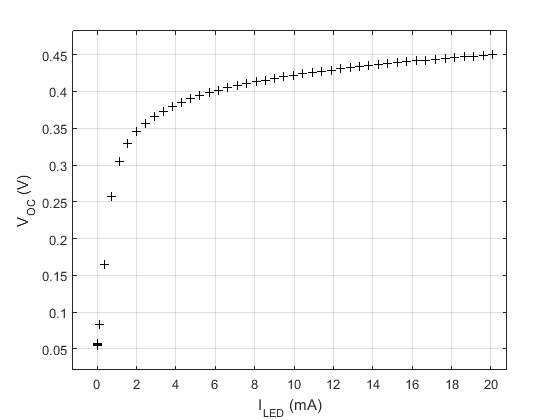
\includegraphics[scale=.6]{es12_1_6-5_50mis}
\caption{Caratteristica $V_{OC}-I_{LED}$ del fotodiodo.}
\label{fig:fotov}
\end{figure}

\subsection{Hm. 4}

Per verificare ciò abbiamo fittato i dati sperimentali tramite fit a due parametri secondo la \ref{eqn:shc}, prendendo k e $V_T$ come parametri liberi. In figura \ref{fig:hm4} è mostrato il grafico di fit, mentre in tabella \ref{tab:fithm4} i risultati del fit stesso. 

\begin{figure}[htp]
\centering
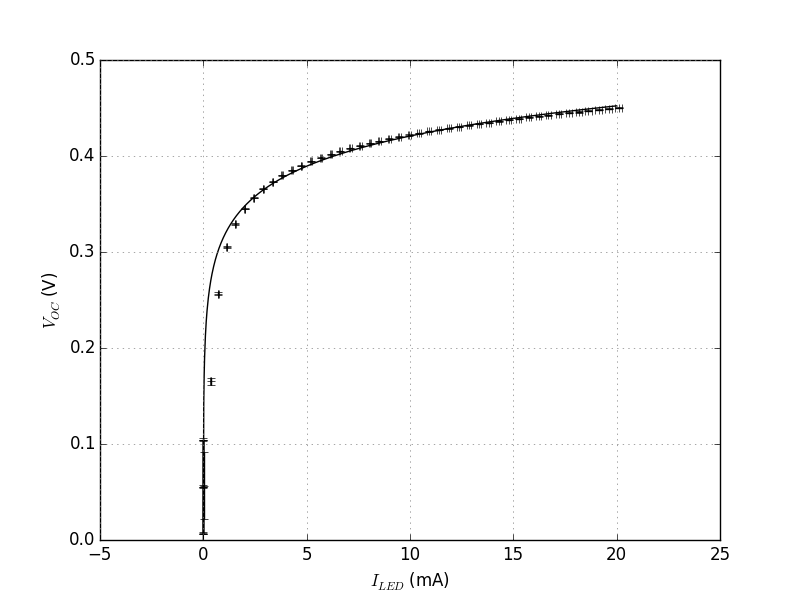
\includegraphics[scale=.4]{hm4}
\caption{Fit caratteristica $V_{OC}-I_{LED}$}
\label{fig:hm4}
\end{figure}

\begin{table}[htp]
\centering
\caption{Parametri del fit}
\label{tab:fithm4}
\begin{tabular}{|c|c|}
\hline 
Parametro & Valore \\ 
\hline 
a & 0.0453(10) V \\ 
\hline 
b & 11(2)$\cdot 10^3$ mA$^{-1}$ \\ 
\hline 
$\chi^2$/ndof & 2055/48 \\ 
\hline 
\end{tabular} 
\end{table}

Come si vede il fit segue abbastanza bene i dati sperimentali, a parte i primi dati, dove però il LED non è più in regime lineare. Se si escludono quindi le prime misure, il fit ottenuto risulta essere quello in figura \ref{fig:hm4_2} e tabella \ref{tab:fit2}. Il grafico risulta maggiormente in accordo con i dati sperimentali e il $\chi^2$ molto più ragionevole, per cui questi valori si possono considerare più significativi dei precedenti.

\begin{figure}[htp]
\centering
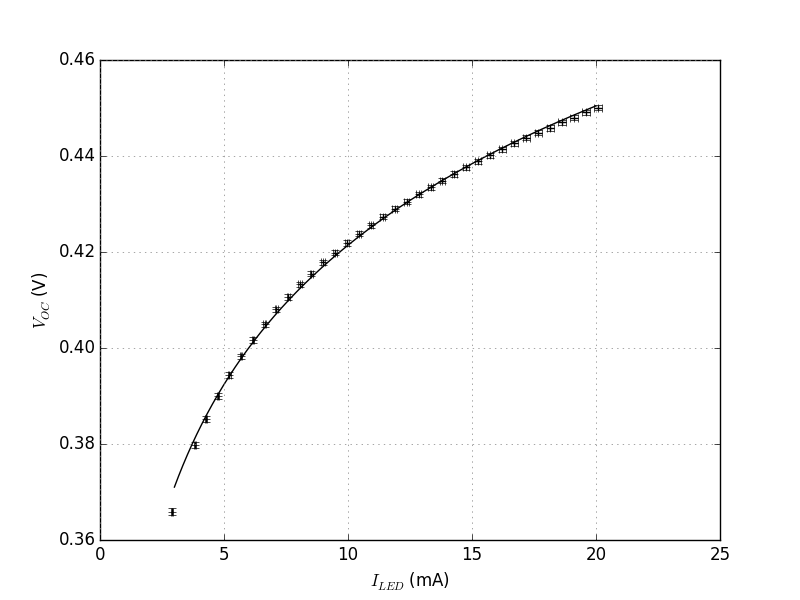
\includegraphics[scale=.4]{hm4_2}
\caption{Fit caratteristica $V_{OC}-I_{LED}$ senza le prime misure.}
\label{fig:hm4_2}
\end{figure}

\begin{table}[htp]
\centering
\caption{Parametri del fit.}
\label{tab:fit2}
\begin{tabular}{|c|c|}
\hline 
Parametro & Valore \\ 
\hline 
a & 0.0419(3) V \\ 
\hline 
b & 235(14) $\cdot 10$ mA$^{-1}$ \\ 
\hline 
$\chi^2$/ndof & 57/34 \\ 
\hline 
\end{tabular} 
\end{table}

\end{document}